\documentclass[chaptersright]{informeutn}
\usepackage{circuitikz}
\usepackage[label=corner]{karnaugh-map}

\materia{Tecnicas Digitales}
\titulo{Trabajo Práctico 1}
\comision{3R2}
\autores{
          Gaston Grasso - 401892\\
          Franco Palombo - 401910\\
      }
\fecha{12/06/2025}

\begin{document}
  \maketitle

  \tableofcontents
  \setcounter{page}{1}
  \thispagestyle{plain}


  \chapter{Conversor de BCD a XS3}
  \begin{figure}[!ht]
    \centering
    \begin{tabular}{|c|c|c|c|c||c|c|c|c|}
    \hline
    \multicolumn{5}{|c||}{Entrada BCD} & \multicolumn{4}{c|}{Salida XS-3} \\
    A & B & C & D & & S3 & S2 & S1 & S0 \\
    \hline
    0 & 0 & 0 & 0 & (0) & 0 & 0 & 1 & 1 \\
    0 & 0 & 0 & 1 & (1) & 0 & 1 & 0 & 0 \\
    0 & 0 & 1 & 0 & (2) & 0 & 1 & 0 & 1 \\
    0 & 0 & 1 & 1 & (3) & 0 & 1 & 1 & 0 \\
    0 & 1 & 0 & 0 & (4) & 0 & 1 & 1 & 1 \\
    0 & 1 & 0 & 1 & (5) & 1 & 0 & 0 & 0 \\
    0 & 1 & 1 & 0 & (6) & 1 & 0 & 0 & 1 \\
    0 & 1 & 1 & 1 & (7) & 1 & 0 & 1 & 0 \\
    1 & 0 & 0 & 0 & (8) & 1 & 0 & 1 & 1 \\
    1 & 0 & 0 & 1 & (9) & 1 & 1 & 0 & 0 \\
    \hline
    \end{tabular}
  \end{figure}
    \begin{minipage}[t]{0.48\textwidth}
      \centering
      \begin{karnaugh-map}[4][4][1][$CD$][$AB$]
        \minterms{5,6,7,8,9}
        \maxterms{0,1,2,3,4}
        \autoterms[X]
        \implicant{5}{15}
        \implicant{7}{14}
        \implicant{12}{10}
      \end{karnaugh-map}
      \captionof{figure}{Mapa de Karnaught para S3}
    \end{minipage}
    \hfill
    \begin{minipage}[t]{0.48\textwidth}
      \centering
      $S3=A+B\cdot(C+D)$
    \end{minipage}
    
    \vspace{1cm}
    
    \noindent
    \begin{minipage}[t]{0.48\textwidth}
      \centering
      \begin{karnaugh-map}[4][4][1][$CD$][$AB$]
        \minterms{1,2,3,4,9}
        \maxterms{0,5,6,7,8}
        \autoterms[X]
        \implicantedge{1}{3}{9}{11}
        \implicantedge{3}{2}{11}{10}
        \implicant{4}{12}
      \end{karnaugh-map}
      \captionof{figure}{Mapa de Karnaught para S2}
    \end{minipage}
    \hfill
    \begin{minipage}[t]{0.48\textwidth}
      \centering
      $S2=\overline{B}\cdot (C +  D) + B \cdot \overline{C} \cdot \overline{D}$
    \end{minipage}
    
    \noindent
    \begin{minipage}[t]{0.48\textwidth}
      \centering
      \begin{karnaugh-map}[4][4][1][$CD$][$AB$]
        \minterms{0,3,4,7,8}
        \maxterms{1,2,5,6,9}
        \autoterms[X]
        \implicant{3}{11}
        \implicant{0}{8}
      \end{karnaugh-map}
      \captionof{figure}{Mapa de Karnaught para S1}
    \end{minipage}
    \hfill
    \begin{minipage}[t]{0.48\textwidth}
      \centering
      $S1=C \cdot D + \overline{C} \cdot \overline{D}$
    \end{minipage}
    
    \noindent
    \begin{minipage}[t]{0.48\textwidth}
      \centering
      \begin{karnaugh-map}[4][4][1][$CD$][$AB$]
        \minterms{0,2,4,6,8}    
        \maxterms{1,3,5,7,9}
        \autoterms[X]
        \implicantedge{0}{8}{2}{10}
      \end{karnaugh-map}
      \captionof{figure}{Mapa de Karnaught para S0}
    \end{minipage}
    \hfill
    \begin{minipage}[t]{0.48\textwidth}
      \centering
      $S0=\overline{D}$
    \end{minipage}

    \section{Implementacion}

     \begin{tikzpicture}
	% Paths, nodes and wires:
	\draw node[ieeestd and port] at (4.378, 12.72) {};
	\draw node[ieeestd or port] at (1.602, 13.53) {};
	\draw node[ieeestd or port] at (6.811, 11.5) {};
	\draw node[ieeestd or port] at (2.189, 7.5) {};
	\draw node[ieeestd and port] at (4.378, 8.72) {};
	\draw node[ieeestd and port] at (2.189, 5.5) {};
	\draw node[ieeestd and port] at (4.5, 4.5) {};
	\draw node[ieeestd or port] at (6.811, 6.5) {};
	\draw node[ieeestd and port] at (2.081, 1.5) {};
	\draw node[ieeestd and port] at (2.081, -0.5) {};
	\draw node[ieeestd or port] at (4.5, 0.5) {};
	\draw node[ieeestd not port, rotate=-90] at (-6, 15.877) {};
	\draw node[ieeestd not port, rotate=-90] at (-4, 15.877) {};
	\draw node[ieeestd not port, rotate=-90] at (-2, 15.877) {};
	\draw node[ieeestd not port, rotate=-90] at (0, 15.877) {};
	\draw (-7, 18) -- (-7, -2);
	\draw (-6, 16.754) |- (-7, 17);
	\draw[draw={rgb,255:red,255;green,0;blue,0}] (-6, 15.219) |- (-6, -2);
	\draw (-5, 18) |- (-5, -2);
	\draw (-3, 18) |- (-3, -2);
	\draw (-1, 18) -- (-1, -2);
	\draw[draw={rgb,255:red,255;green,0;blue,0}] (-2, 15.219) -| (-2, -2);
	\draw[draw={rgb,255:red,255;green,0;blue,0}] (0, 15.219) -- (0, -2);
	\draw[draw={rgb,255:red,255;green,0;blue,0}] (-4, 15.219) |- (-4, -2);
	\draw (-4, 16.754) |- (-5, 17);
	\draw (-2, 16.754) |- (-3, 17);
	\draw (0, 16.754) |- (-1, 17);
	\draw node[circ] (N1) at (-7, 18) {} node[anchor=south] at (N1.north){$A$};
	\draw node[circ] (N2) at (-5, 18) {} node[anchor=south] at (N2.north){$B$};
	\draw node[circ] (N3) at (-3, 18) {} node[anchor=south] at (N3.north){$C$};
	\draw node[circ] (N4) at (-1, 18) {} node[anchor=south] at (N4.north){$D$};
	\draw node[circ] at (-1, 13.25) {};
	\draw node[circ] at (-3, 13.81) {};
	\draw node[circ] at (-5, 12.44) {};
	\draw node[circ] at (-7, 11.19) {};
	\draw node[circ] at (-4, 9) {};
	\draw node[circ] at (-3, 7.78) {};
	\draw node[circ] at (-1, 7.22) {};
	\draw node[circ] at (-2, 5.22) {};
	\draw node[circ] at (-5, 5.78) {};
	\draw node[circ] at (0, 4.22) {};
	\draw node[circ] at (-3, 1.78) {};
	\draw node[circ] at (-1, 1.22) {};
	\draw node[circ] at (-2, -0.22) {};
	\draw node[circ] at (0, -0.78) {};
	\draw node[circ] at (0, -2) {};
	\draw node[circ] (N5) at (8.5, 11.5) {} node[anchor=west] at (N5.east){$S3$};
	\draw node[circ] (N6) at (8.5, 6.53) {} node[anchor=west] at (N6.east){$S2$};
	\draw node[circ] (N7) at (8.5, 0.53) {} node[anchor=west] at (N7.east){$S1$};
	\draw node[circ] (N8) at (8.5, -2) {} node[anchor=west] at (N8.east){$S0$};
	\draw (3.46, 9) -- (3.568, 9);
	\draw (3.162, -0.5) -- (3.27, -0.5);
	\draw (0.52, 13.81) -| (-3, 14);
	\draw (0.52, 13.25) -| (-1, 13.5) -| (-1, 13);
	\draw (3.297, 13) |- (2.683, 13.53);
	\draw (3.297, 12.44) -| (-5, 12.5);
	\draw (5.73, 11.78) |- (5.46, 12.72);
	\draw (5.73, 11.22) -| (-7, 11);
	\draw (3.297, 9) -| (-4, 9);
	\draw (1.108, 7.78) -| (-3, 7.5);
	\draw (1.108, 7.22) -| (-1, 7);
	\draw (3.27, 7.5) |- (3.297, 8.44);
	\draw (5.46, 8.72) -| (5.73, 6.78);
	\draw (5.5, 4.5) -| (5.73, 6.22);
	\draw (3.419, 4.78) |- (3.27, 5.5);
	\draw (3.419, 4.22) -| (0, 4);
	\draw (1.108, 5.78) -| (-5, 5.5);
	\draw (1.108, 5.22) -| (-2, 5);
	\draw (1, 1.78) -| (-3, 1.5);
	\draw (1, 1.22) -| (-1, 1.5);
	\draw (3.162, 1.5) -| (3.419, 0.78);
	\draw (3.419, 0.22) |- (3.27, -0.5);
	\draw (1, -0.22) -| (-2, -0.5) -- (-2, -0);
	\draw (1, -0.78) -| (0, -0.5);
	\draw (8.5, -2) -- (-0, -2);
	\draw (5.581, 0.5) -| (8.5, 0.5);
	\draw (7.892, 6.5) -| (8.5, 6.5);
	\draw (7.892, 11.5) -- (8.5, 11.5);
\end{tikzpicture}
    
  \chapter{Comparador binario}
    Para el comparador binario, hay dos conjuntos de entradas de dos bits, y tres salidas, que ambas dependen de los
    dos conjuntos de entradas. La tabla de verdad del comparador binario es la de la figura (\ref{tt.bin.comp}).
    \begin{figure}[!ht]
      \centering
      \begin{tabular}{|c|c|c|c|c|c||c|c|c|c|c|}
        \hline
        \multicolumn{4}{|c}{Entradas} & \multicolumn{2}{|c||}{Num.} & \multicolumn{4}{c|}{Salidas} \\
        $A_1$ & $A_0$ & $B_1$ & $B_0$ & A & B & $S_2$ & $S_1$ & $S_0$ &\\
        \hline
        0     & 0     & 0     & 0     & 0 & 0 & 1     & 0     & 0     & $A=B$\\
        0     & 0     & 0     & 1     & 0 & 1 & 0     & 1     & 0     & $A<B$\\
        0     & 0     & 1     & 0     & 0 & 2 & 0     & 1     & 0     & $A<B$\\
        0     & 0     & 1     & 1     & 0 & 3 & 0     & 1     & 0     & $A<B$\\
        0     & 1     & 0     & 0     & 1 & 0 & 0     & 0     & 1     & $A>B$\\
        0     & 1     & 0     & 1     & 1 & 1 & 1     & 0     & 0     & $A=B$\\
        0     & 1     & 1     & 0     & 1 & 2 & 0     & 1     & 0     & $A<B$\\
        0     & 1     & 1     & 1     & 1 & 3 & 0     & 1     & 0     & $A<B$\\
        1     & 0     & 0     & 0     & 2 & 0 & 0     & 0     & 1     & $A>B$\\
        1     & 0     & 0     & 1     & 2 & 1 & 0     & 0     & 1     & $A>B$\\
        1     & 0     & 1     & 0     & 2 & 2 & 1     & 0     & 0     & $A=B$\\
        1     & 0     & 1     & 1     & 2 & 3 & 0     & 1     & 0     & $A<B$\\
        1     & 1     & 0     & 0     & 3 & 0 & 0     & 0     & 1     & $A>B$\\
        1     & 1     & 0     & 1     & 3 & 1 & 0     & 0     & 1     & $A>B$\\
        1     & 1     & 1     & 0     & 3 & 2 & 0     & 0     & 1     & $A>B$\\
        1     & 1     & 1     & 1     & 3 & 3 & 1     & 0     & 0     & $A=B$\\
        \hline
      \end{tabular}
      \caption{Tabla de verdad del comparador binario}
      \label{tt.bin.comp}
    \end{figure}

    Los mapas de karnaugh para las funciones $S_2$, $S_1$ y $S_0$ son los de las figuras (\ref{km.bin.comp.s2}),
    (\ref{km.bin.comp.s1}) y (\ref{km.bin.comp.s0}) respectivamente.

    \begin{figure}[!ht]
      \centering
      \begin{minipage}[t]{0.48\textwidth}
        \centering
        \begin{karnaugh-map}[4][4][1][$B_0$][$B_1$][$A_0$][$A_1$]
          \minterms{4,8,9,12,13,14}
          \implicant{4}{12}
          \implicant{12}{9}
          \implicantedge{12}{12}{14}{14}
        \end{karnaugh-map}
        \vspace{-5mm}
        \begin{equation*}
          S_0 = A_1 \, \overline{B_1} + A_0 \, \overline{B_1} \, \overline{B_0} + A_1 \, A_0 \, \overline{B_0}
        \end{equation*}
        \caption{Mapa de Karnaugh para $S_0$}
        \label{km.bin.comp.s0}
      \end{minipage}
      \begin{minipage}[t]{0.48\textwidth}
        \centering
        \begin{karnaugh-map}[4][4][1][$B_0$][$B_1$][$A_0$][$A_1$]
          \minterms{1,2,3,6,7,11}
          \implicant{3}{6}
          \implicant{1}{3}
          \implicantedge{3}{3}{11}{11}
        \end{karnaugh-map}
        \vspace{-5mm}
        \begin{equation*}
          S_1 = \overline{A_1} \, B_1 + \overline{A_1} \, \overline{A_0} \, B_0 + \overline{A_0} \, B_1 \, B_0
        \end{equation*}
        \caption{Mapa de Karnaugh para $S_1$}
        \label{km.bin.comp.s1}
      \end{minipage}
      \begin{minipage}[t]{1\textwidth}
        \vspace{5mm}
        \centering
        \begin{karnaugh-map}[4][4][1][$B_0$][$B_1$][$A_0$][$A_1$]
          \minterms{0,5,10,15}
          \implicant{0}{0}
          \implicant{5}{5}
          \implicant{10}{10}
          \implicant{15}{15}
        \end{karnaugh-map}
        \vspace{-5mm}
        \begin{gather*}
          S_2 = \overline{A_1} \, \overline{A_0} \, \overline{B_1} \, \overline{B_0} + \overline{A_1} \, A_0 \,
                \overline{B_1} \, B_0 + A_1 \, A_0 \, B_1 \, B_0 + A_1 \, \overline{A_0} \, B_1 \, \overline{B_0}\\[6pt]
          S_2 = \overline{S_0} \, \overline{S_1}
        \end{gather*}
        \caption{Mapa de Karnaugh para $S_2$}
        \label{km.bin.comp.s2}
      \end{minipage}
    \end{figure}

    La funcion booleana para $S_2$ se puede simplificar utilizando las salidas $S_0$ y $S_1$. Ya que estas nunca van
    a ser igual a 1 en simultaneo, pero, si van a ser igual a 0 en simultaneo. El caso en el que A no es mayor que B y
    B tampoco es mayor que A, es cuando A y B son iguales, por lo que podriamos tomar las salidas $\overline{S_0}$ y
    $\overline{S_1}$ y pasarlas por una compuerta AND para que produzcan el mismo resultado que la simplificacion de
    Karnaugh, pero con muchas menos compuertas.

    Se implemento las operaciones booleanas tal y como estan en la figura (\ref{crkt.ej2}), utilizando compuertas AND
    de 2 entradas y OR de 2 entradas. En la figura (\ref{falstad.ej2}) se puede ver el circuito implementado en Falstad
    como se va a implementar en la protoboard en base a las compuertas disponibles y comodidad de armado.

    \begin{figure}[!ht]
      \centering
      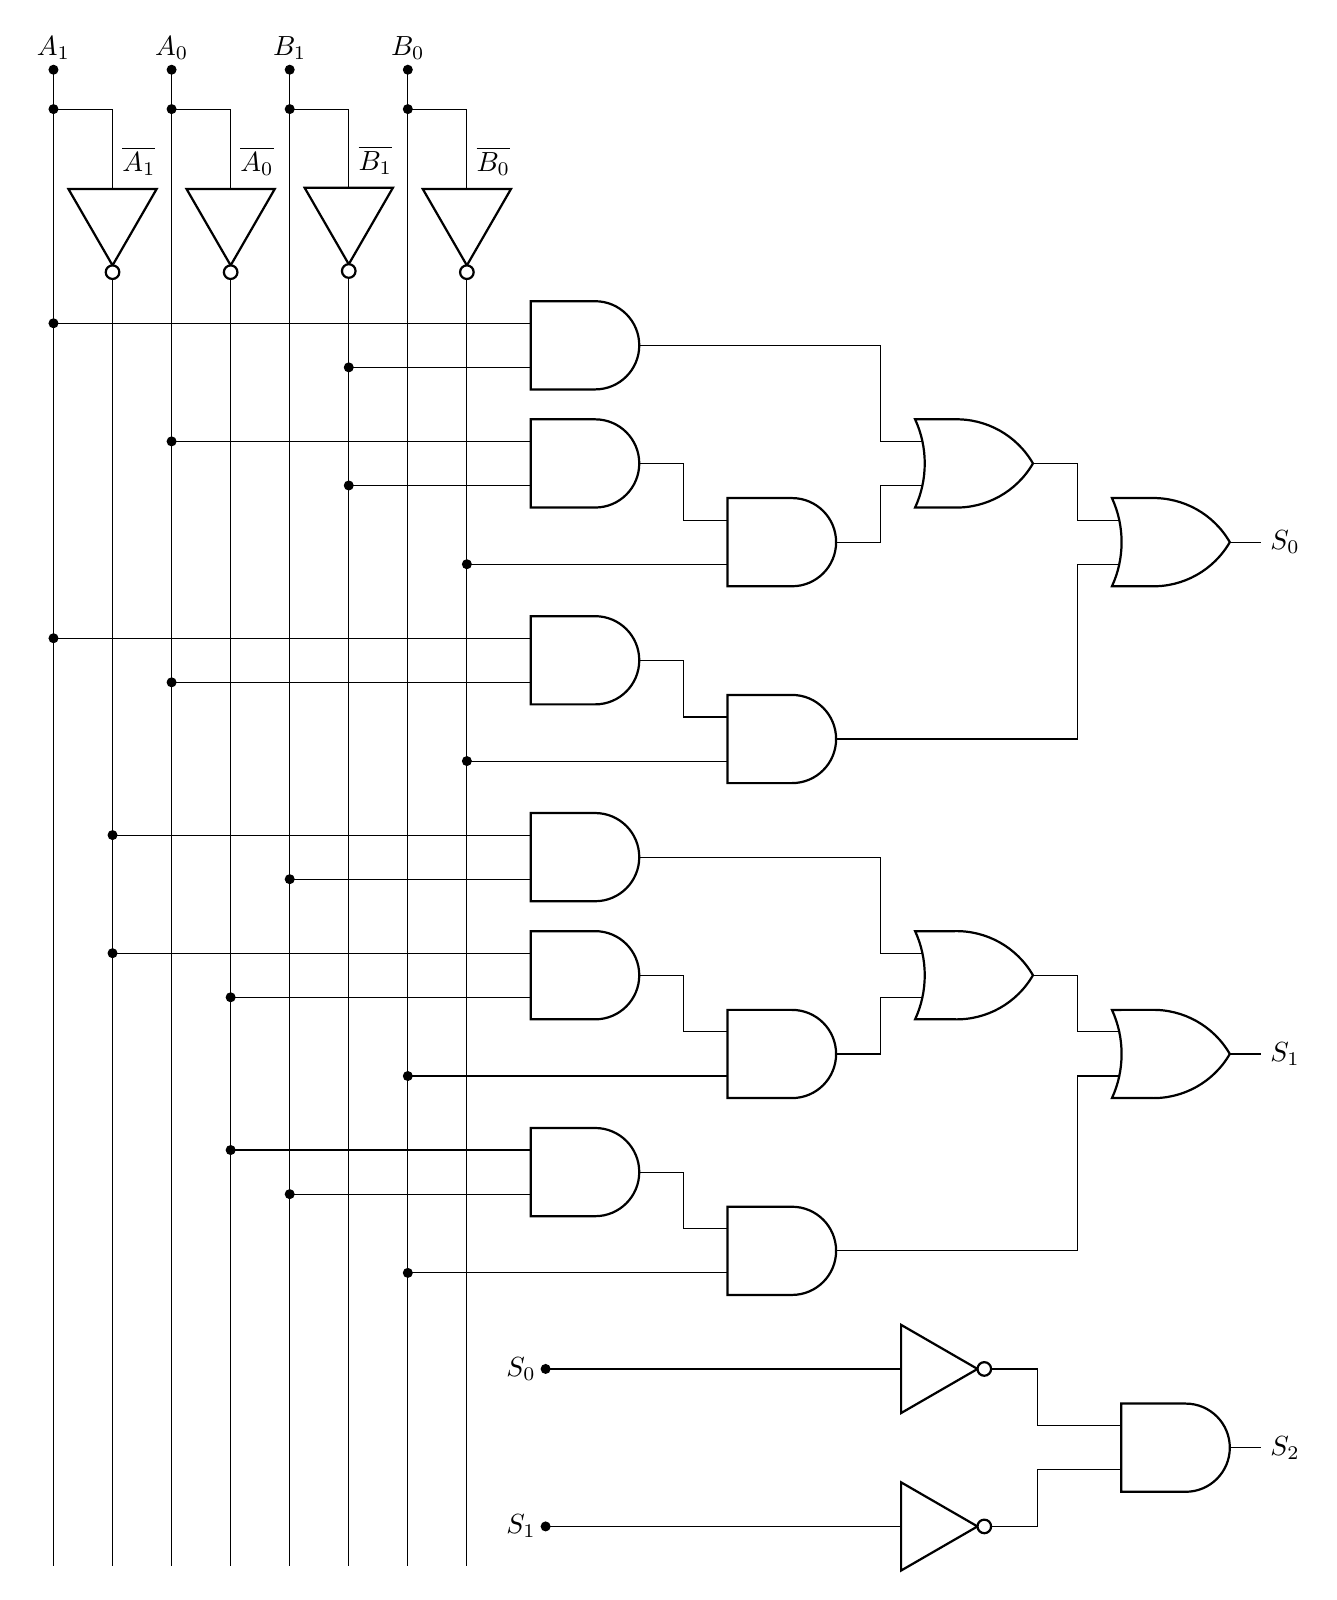
\begin{tikzpicture}
        % Paths, nodes and wires:
        \draw node[ieeestd not port, rotate=-90] (N1) at (4, 10) {} node[anchor=west] at ([yshift=3.5mm]N1.west){$\overline{A_0}$};
        \draw node[ieeestd not port, rotate=-90] (N2) at (5.5, 10.015) {} node[anchor=west] at ([yshift=3.5mm]N2.west){$\overline{B_1}$};
        \draw node[ieeestd not port, rotate=-90] (N3) at (7, 10) {} node[anchor=west] at ([yshift=3.5mm]N3.west){$\overline{B_0}$};
        \draw node[ieeestd not port, rotate=-90] (N4) at (2.5, 10) {} node[anchor=west] at ([yshift=3.5mm]N4.west){$\overline{A_1}$};
        \draw node[ieeestd and port] at (8.5, 2) {};
        \draw node[ieeestd and port] at (8.5, 0.5) {};
        \draw node[ieeestd and port] at (8.5, -2) {};
        \draw node[ieeestd or port] at (13.5, 0.5) {};
        \draw node[ieeestd or port] (N5) at (16, -0.5) {} node[anchor=west] at (N5.east){$S_1$};
        \draw node[ieeestd and port] at (11, -0.5) {};
        \draw node[ieeestd and port] at (11, -3) {};
        \draw (2.5, 10.877) -| (2.5, 11.5) -- (1.75, 11.5);
        \draw (4, 10.877) -- (4, 11.5) -- (3.25, 11.5);
        \draw (5.5, 10.892) -- (5.5, 11.5) -- (4.75, 11.5);
        \draw (7, 10.877) -- (7, 11.5) -| (6.25, 11.5);
        \draw (7.419, 8.78) -| (1.75, 8.75);
        \draw (7.419, 8.22) -| (5.5, 8.25);
        \draw (7.419, 7.28) -| (3.25, 7.25);
        \draw (7.419, 6.72) -| (5.5, 6.75);
        \draw (7.419, 4.78) -| (1.75, 4.75);
        \draw (7.419, 4.22) -| (3.25, 4.25);
        \draw node[circ] at (4.75, 11.5) {};
        \draw node[circ] at (6.25, 11.5) {};
        \draw node[circ] at (3.25, 11.5) {};
        \draw node[circ] at (1.75, 11.5) {};
        \draw node[circ] (N6) at (1.75, 12) {} node[anchor=south] at (N6.text){$A_1$};
        \draw node[circ] (N7) at (3.25, 12) {} node[anchor=south] at (N7.text){$A_0$};
        \draw node[circ] (N8) at (4.75, 12) {} node[anchor=south] at (N8.text){$B_1$};
        \draw node[circ] (N9) at (6.25, 12) {} node[anchor=south] at (N9.text){$B_0$};
        \draw (7.419, 2.28) -| (2.5, 2.25);
        \draw (7.419, 1.72) |- (4.75, 1.72);
        \draw (7.419, 0.78) -| (2.5, 0.75);
        \draw (7.419, 0.22) -| (4, 0.25);
        \draw (9.919, -0.78) |- (6.25, -0.78);
        \draw (7.419, -1.72) -- (4, -1.72);
        \draw (7.419, -2.28) -| (4.75, -2.25);
        \draw (9.919, -3.28) -| (6.25, -3.25);
        \draw node[ieeestd and port] (N10) at (16, -5.5) {} node[anchor=west] at (N10.east){$S_2$};
        \draw node[ieeestd not port] at (13, -4.5) {};
        \draw node[ieeestd not port] at (13, -6.5) {};
        \draw (14.919, -5.22) -| (14.25, -4.5) -- (13.877, -4.5);
        \draw (14.919, -5.78) -| (14.25, -6.5) -- (13.877, -6.5);
        \draw (12.123, -4.5) -- (8, -4.5);
        \draw (12.123, -6.5) -- (8, -6.5);
        \draw node[circ] (N11) at (8, -4.5) {} node[anchor=east] at (N11.text){$S_0$};
        \draw node[circ] (N12) at (8, -6.5) {} node[anchor=east] at (N12.text){$S_1$};
        \draw (9.919, -0.22) -| (9.75, 0.5) |- (9.581, 0.5);
        \draw (9.919, -2.72) -| (9.75, -2) |- (9.581, -2);
        \draw (12.419, 0.22) -| (12.25, -0.5) |- (12.081, -0.5);
        \draw (12.419, 0.78) -| (12.25, 2) |- (9.581, 2);
        \draw (14.919, -0.22) -| (14.75, 0.5) |- (14.581, 0.5);
        \draw (14.919, -0.78) -| (14.75, -3) |- (12.081, -3);
        \draw node[ieeestd and port] at (8.5, 8.5) {};
        \draw node[ieeestd and port] at (8.5, 7) {};
        \draw node[ieeestd and port] at (8.5, 4.5) {};
        \draw node[ieeestd or port] at (13.5, 7) {};
        \draw node[ieeestd or port] (N13) at (16, 6) {} node[anchor=west] at (N13.east){$S_0$};
        \draw node[ieeestd and port] at (11, 6) {};
        \draw node[ieeestd and port] at (11, 3.5) {};
        \draw (9.919, 6.28) -| (9.75, 7) |- (9.581, 7);
        \draw (9.919, 3.78) -| (9.75, 4.5) |- (9.581, 4.5);
        \draw (12.419, 6.72) -| (12.25, 6) |- (12.081, 6);
        \draw (12.419, 7.28) -| (12.25, 8.5) |- (9.581, 8.5);
        \draw (14.919, 6.28) -| (14.75, 7) |- (14.581, 7);
        \draw (14.919, 5.72) -| (14.75, 3.5) |- (12.081, 3.5);
        \draw (9.919, 5.72) -| (7, 5.75);
        \draw (9.919, 3.22) -| (7, 3.25);
        \draw (7, 9.123) -- (7, -7);
        \draw (6.25, 12) -- (6.25, -7);
        \draw (4.75, 12) -- (4.75, -7);
        \draw (3.25, 12) -- (3.25, -7);
        \draw (1.75, 12) -- (1.75, -7);
        \draw (2.5, 9.123) -- (2.5, -7);
        \draw (4, 9.123) -- (4, -7);
        \draw (5.5, 9.138) -- (5.5, -7);
        \draw node[circ] at (1.75, 8.78) {};
        \draw node[circ] at (3.25, 7.28) {};
        \draw node[circ] at (5.5, 8.22) {};
        \draw node[circ] at (5.5, 6.72) {};
        \draw node[circ] at (7, 5.72) {};
        \draw node[circ] at (1.75, 4.78) {};
        \draw node[circ] at (3.25, 4.22) {};
        \draw node[circ] at (7, 3.22) {};
        \draw node[circ] at (2.5, 2.28) {};
        \draw node[circ] at (4.75, 1.72) {};
        \draw node[circ] at (2.5, 0.78) {};
        \draw node[circ] at (4, 0.22) {};
        \draw node[circ] at (6.25, -0.78) {};
        \draw node[circ] at (4, -1.72) {};
        \draw node[circ] at (4.75, -2.28) {};
        \draw node[circ] at (6.25, -3.28) {};
      \end{tikzpicture}
      \caption{Implementacion del Comparador binario.}
      \label{crkt.ej2}
    \end{figure}

    \begin{figure}[!ht]
      \centering
      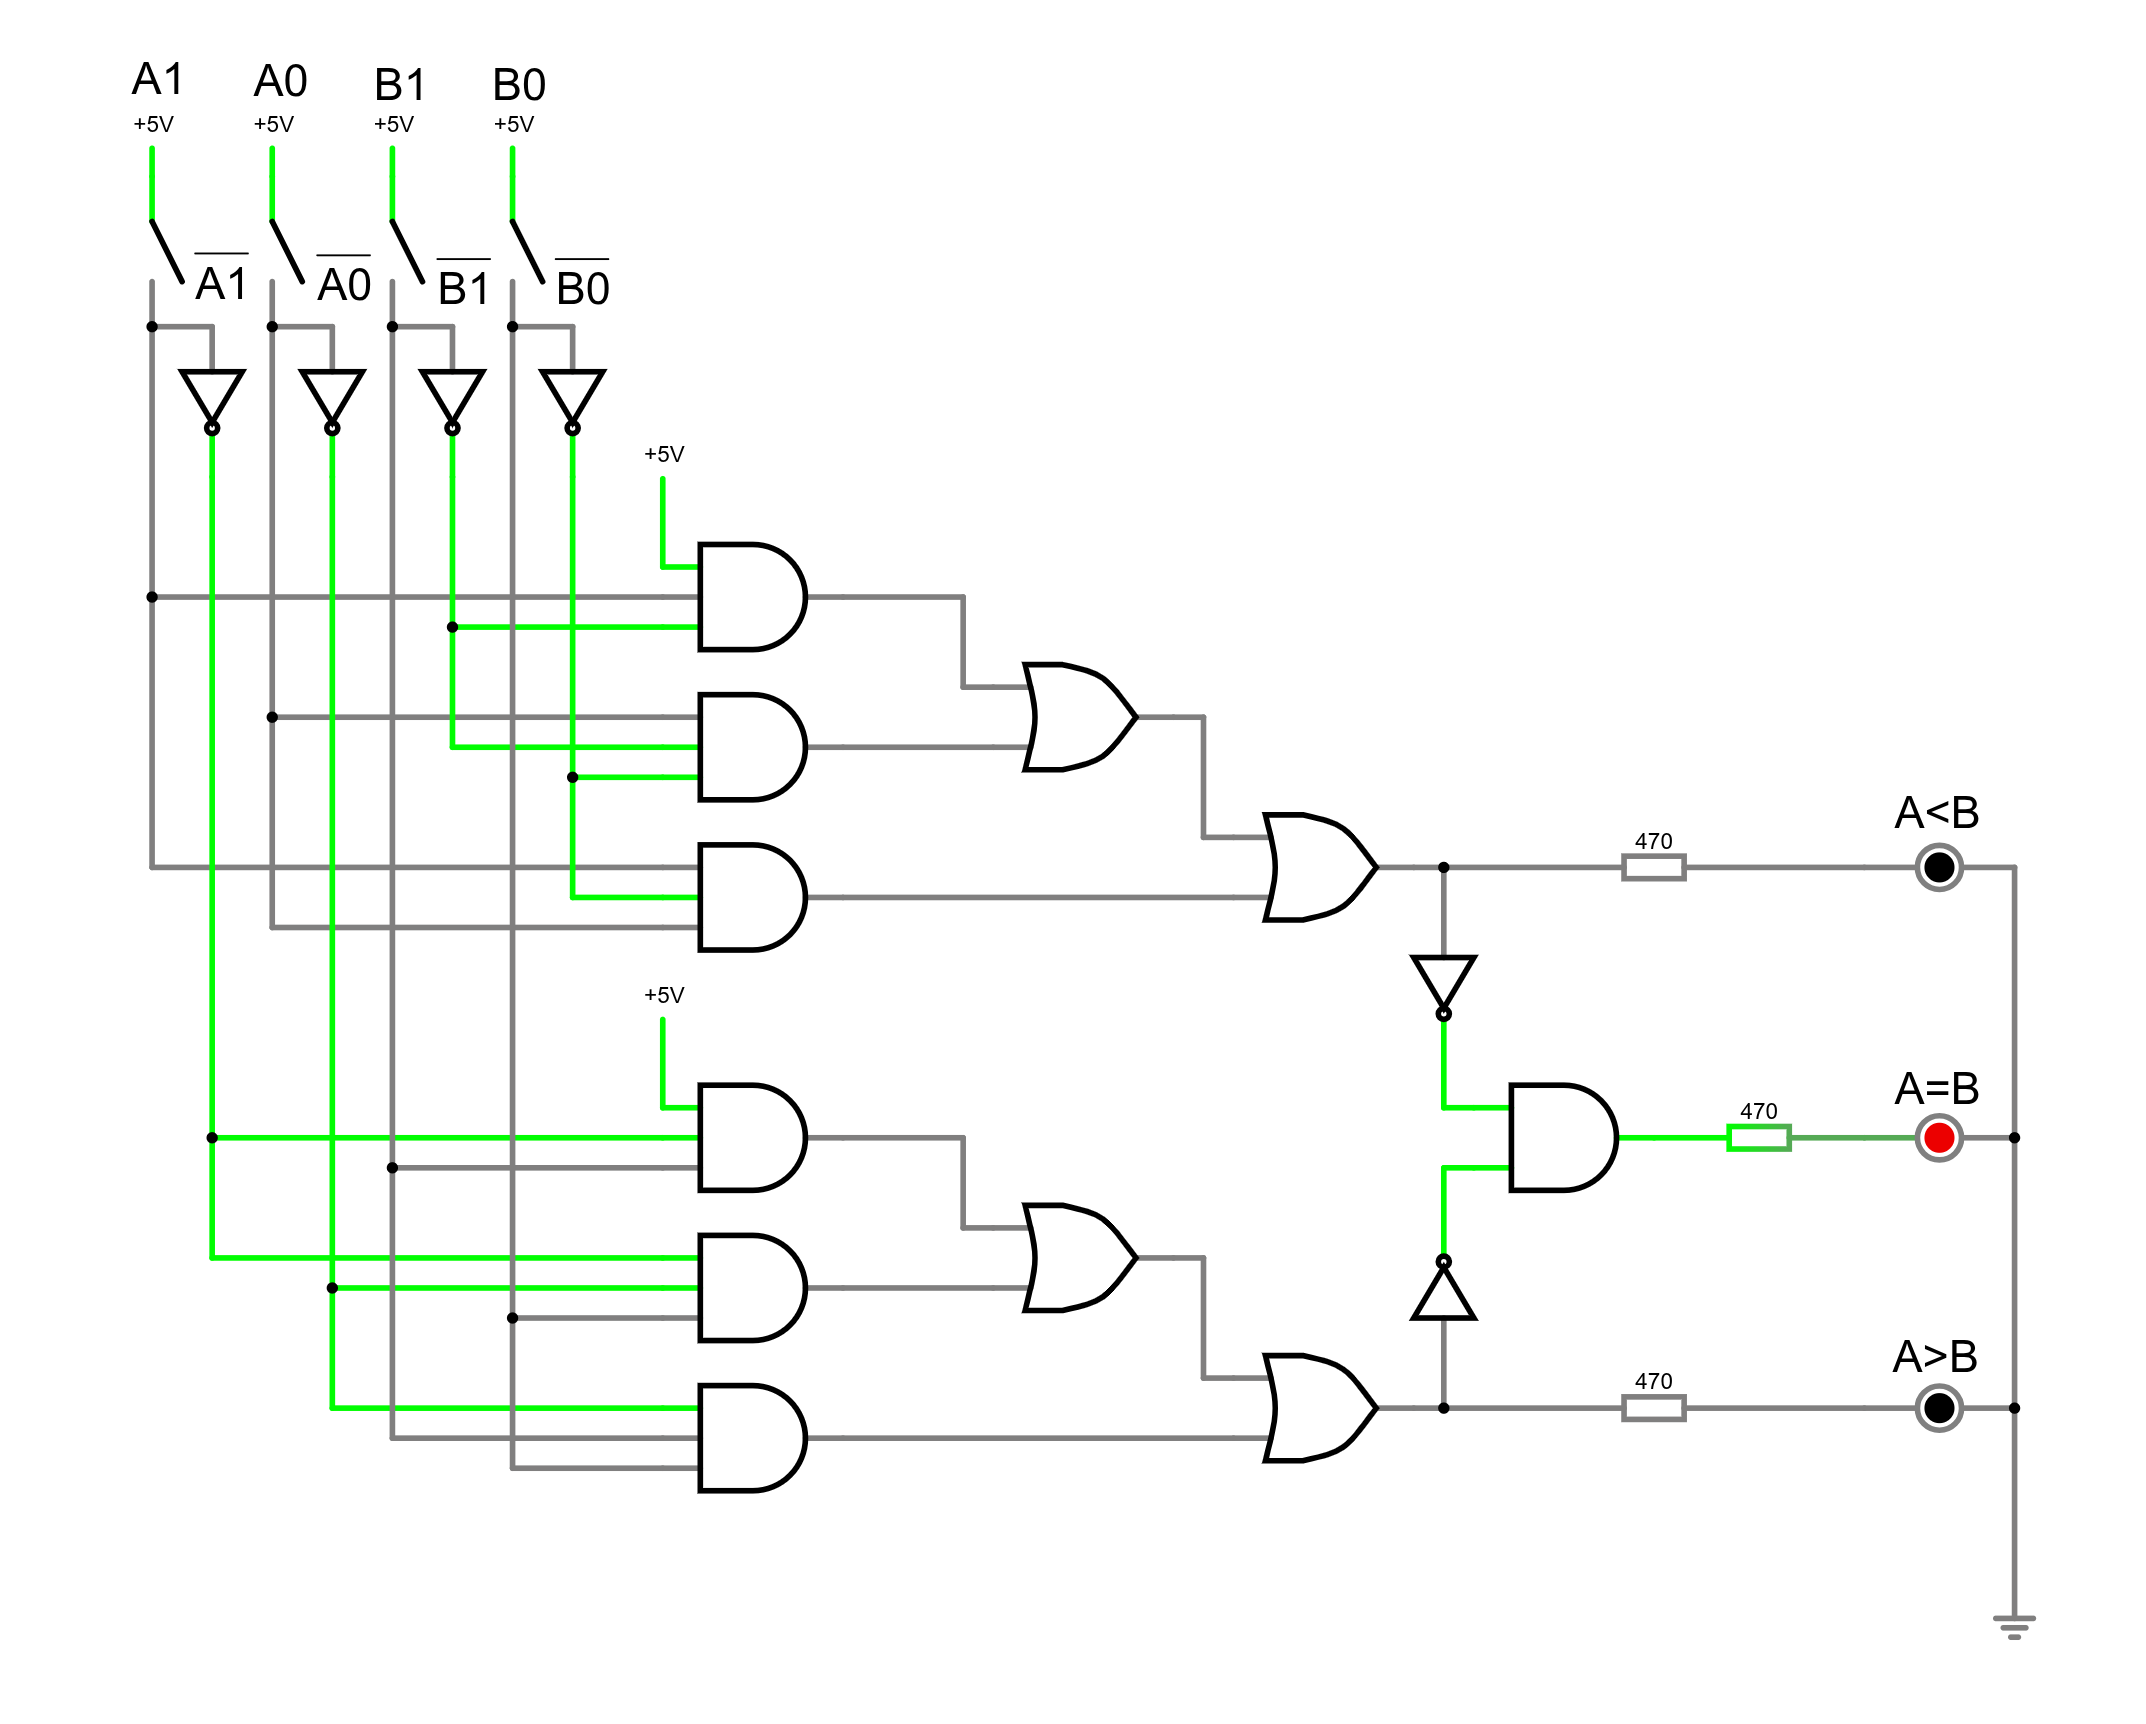
\includegraphics[width=1\textwidth]{images/ej2.png}
      \caption{Implementacion del Comparador binario en Falstad.}
      \label{falstad.ej2}
    \end{figure}

    En la figura (\ref{crkt.ej2.prot}) se puede ver el circuito implementado en la protoboard, utilizando los IC CD4081
    (AND2), CD4073 (AND3), CD4049 (NOT6) y HEF4071 (OR2).

    \begin{figure}[!ht]
      \centering
      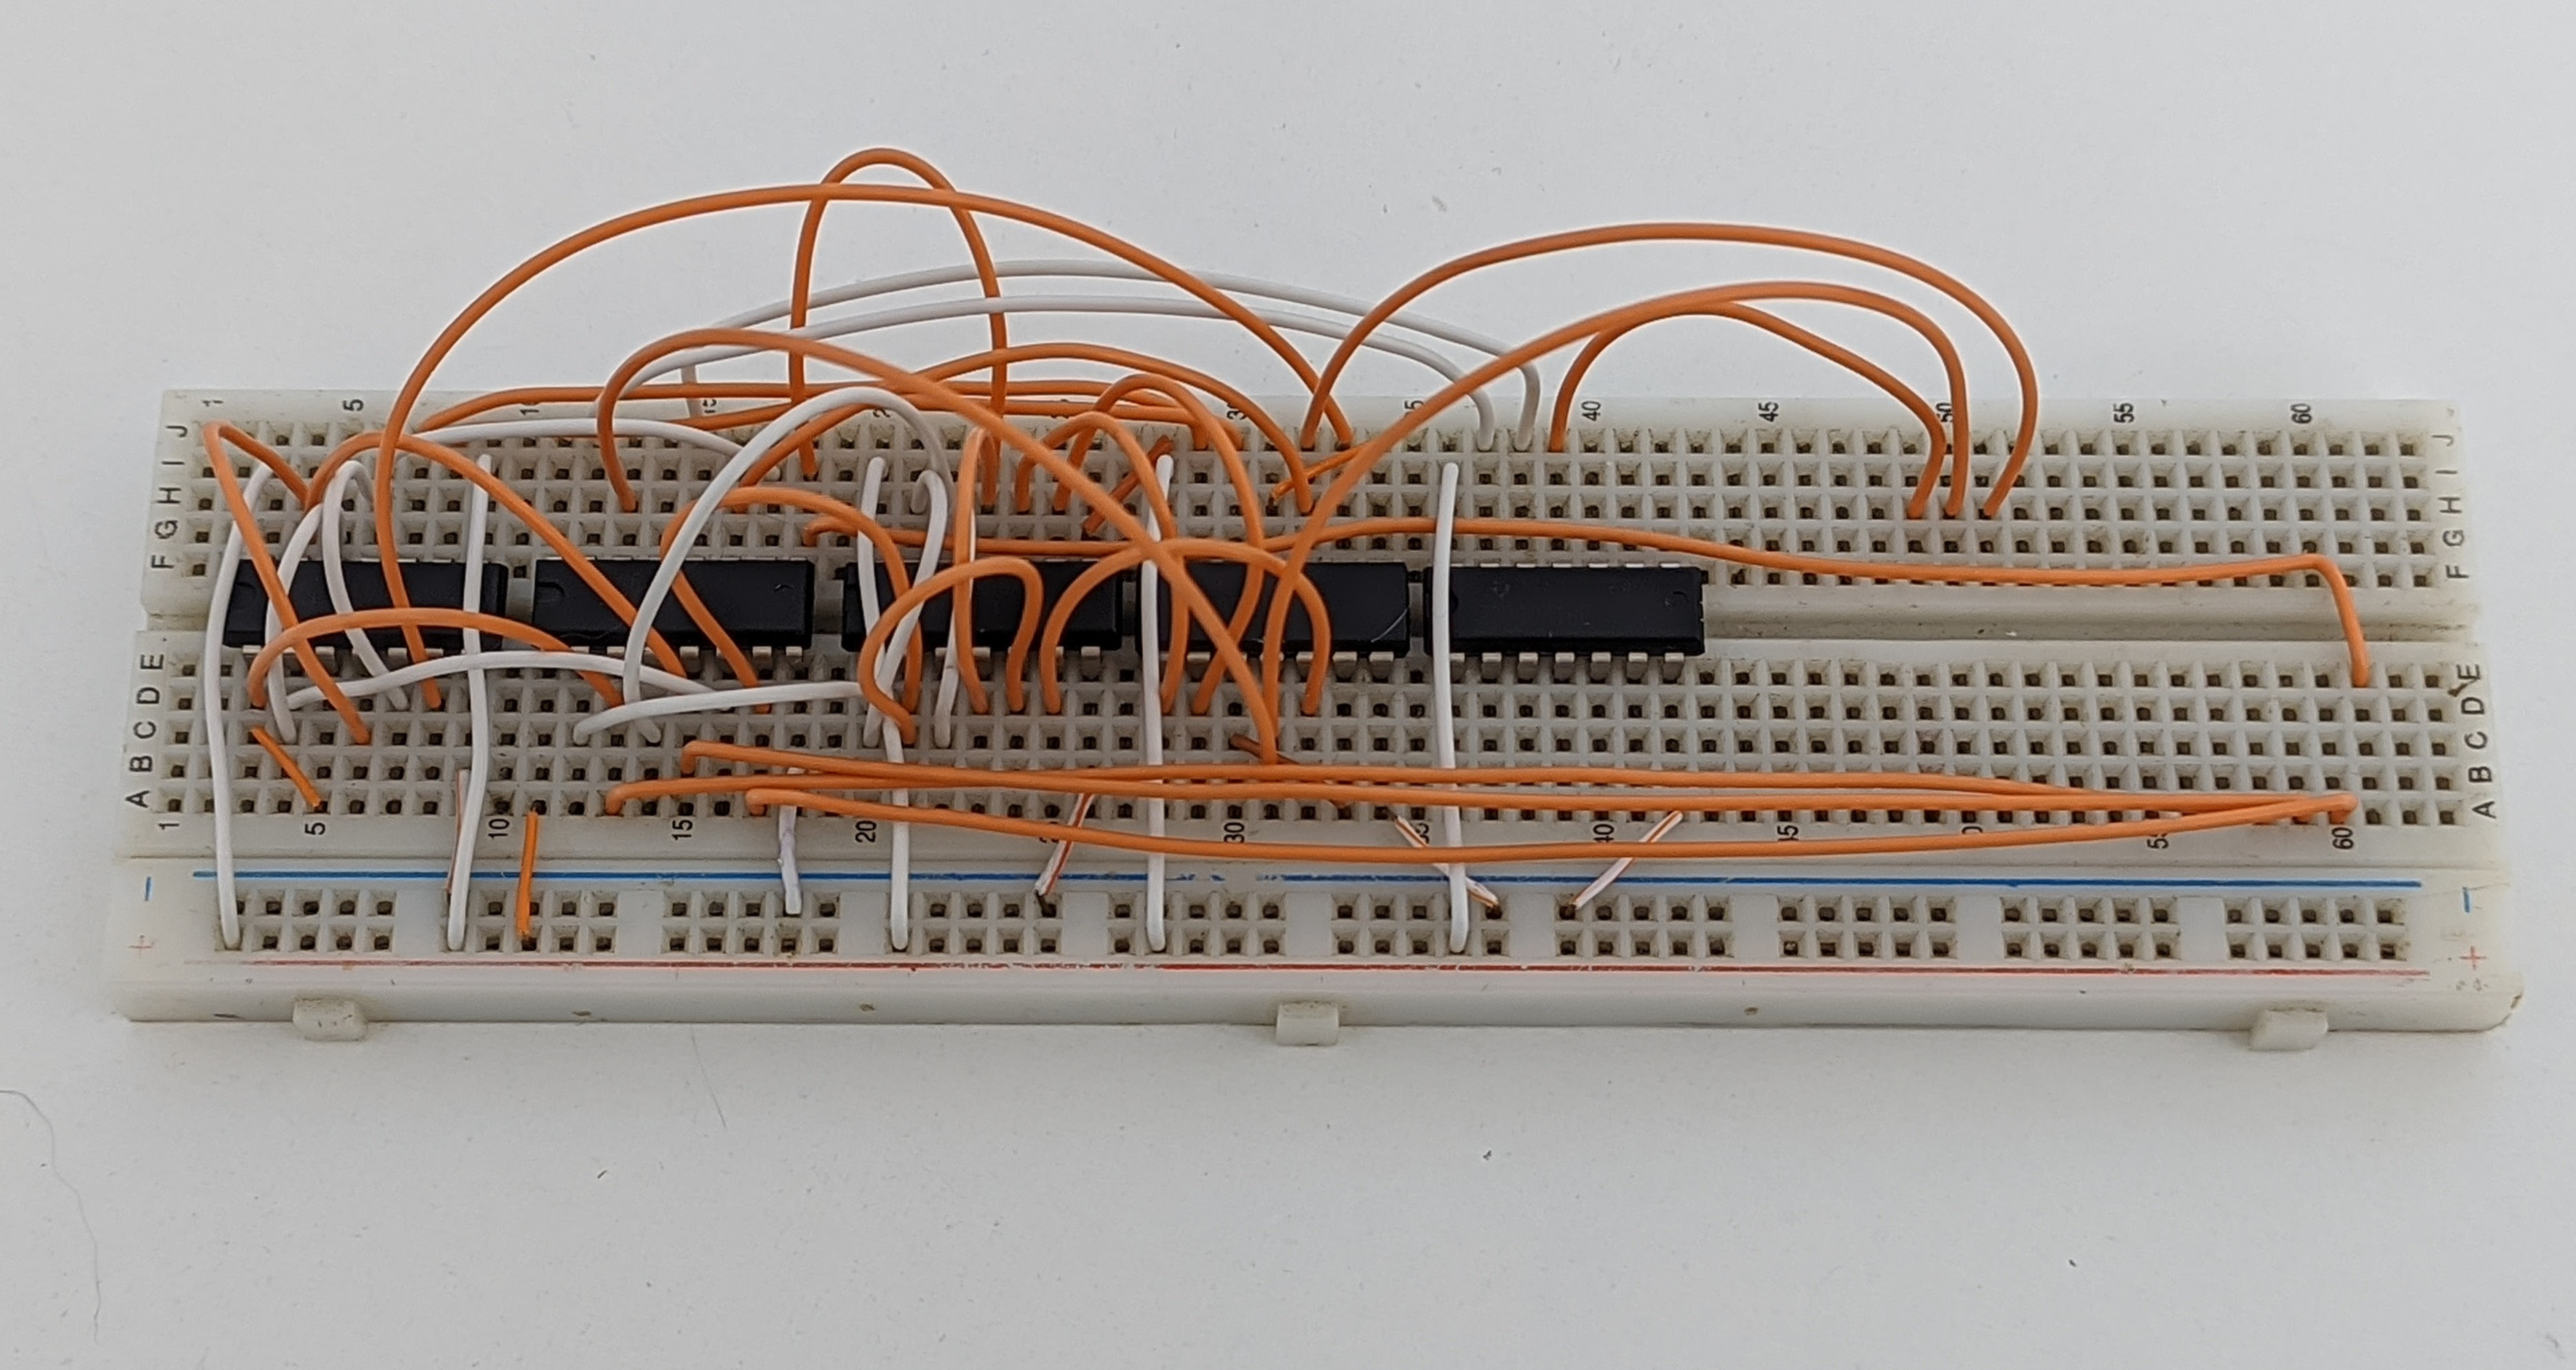
\includegraphics[width=.8\textwidth]{pictures/prot-ej2.jpg}
      \caption{Implementacion del Comparador binario en la protoboard.}
      \label{crkt.ej2.prot}
    \end{figure}


\end{document}

